\section{Reale Ist-Prozesse}\label{sec:realeIst}
In diesem Kapitel sollen weitere Wagenarten und auch unterschiedliche Ladungen angeschnitten werden.\par
Im ersten Teil im Anhang soll es um Kesselwagen auf dem Betriebsgelände der IDR (Industrieterrains Düsseldorf-Reisholz AG) gehen. Diese werden sowohl mit Gefahrgut als auch mit ''normalen'' Chemikalien gefüllt. Die hier abgebildeten Prozesse entsprechen nur der Abwicklung auf dem Betriebsgelände und sind aus einer Interview mit dem EBL extrahiert worden. Auf dem Betriebsgelände werden die Wagen, auch wenn sie später als Ganzzug das Werk verlassen wie Einzelwagen oder kleine Wagengruppen behandelt. Die hier beschriebenen Prozesse zeigen vor allem die Disposition. Die Kupplungsvorgänge, technischen Wagenbehandlungen und Bremsproben entsprechen grob denen bereits beschriebenen.
\subsection{Kessenwagen auf dem Betriebsgelände}
\textbf{Hier Prozess beschreiben}
\begin{figure}
    \centering
    % Define block styles
\tikzstyle{block} = [rectangle, fill=blue!20, text width=5em, text centered, rounded corners, minimum height=4em, text width=8em]
\tikzstyle{cloud} = [draw, rectangle, fill=gray!20, node distance=2.5cm, minimum height=2em]
\tikzstyle{invisible} = [rectangle]


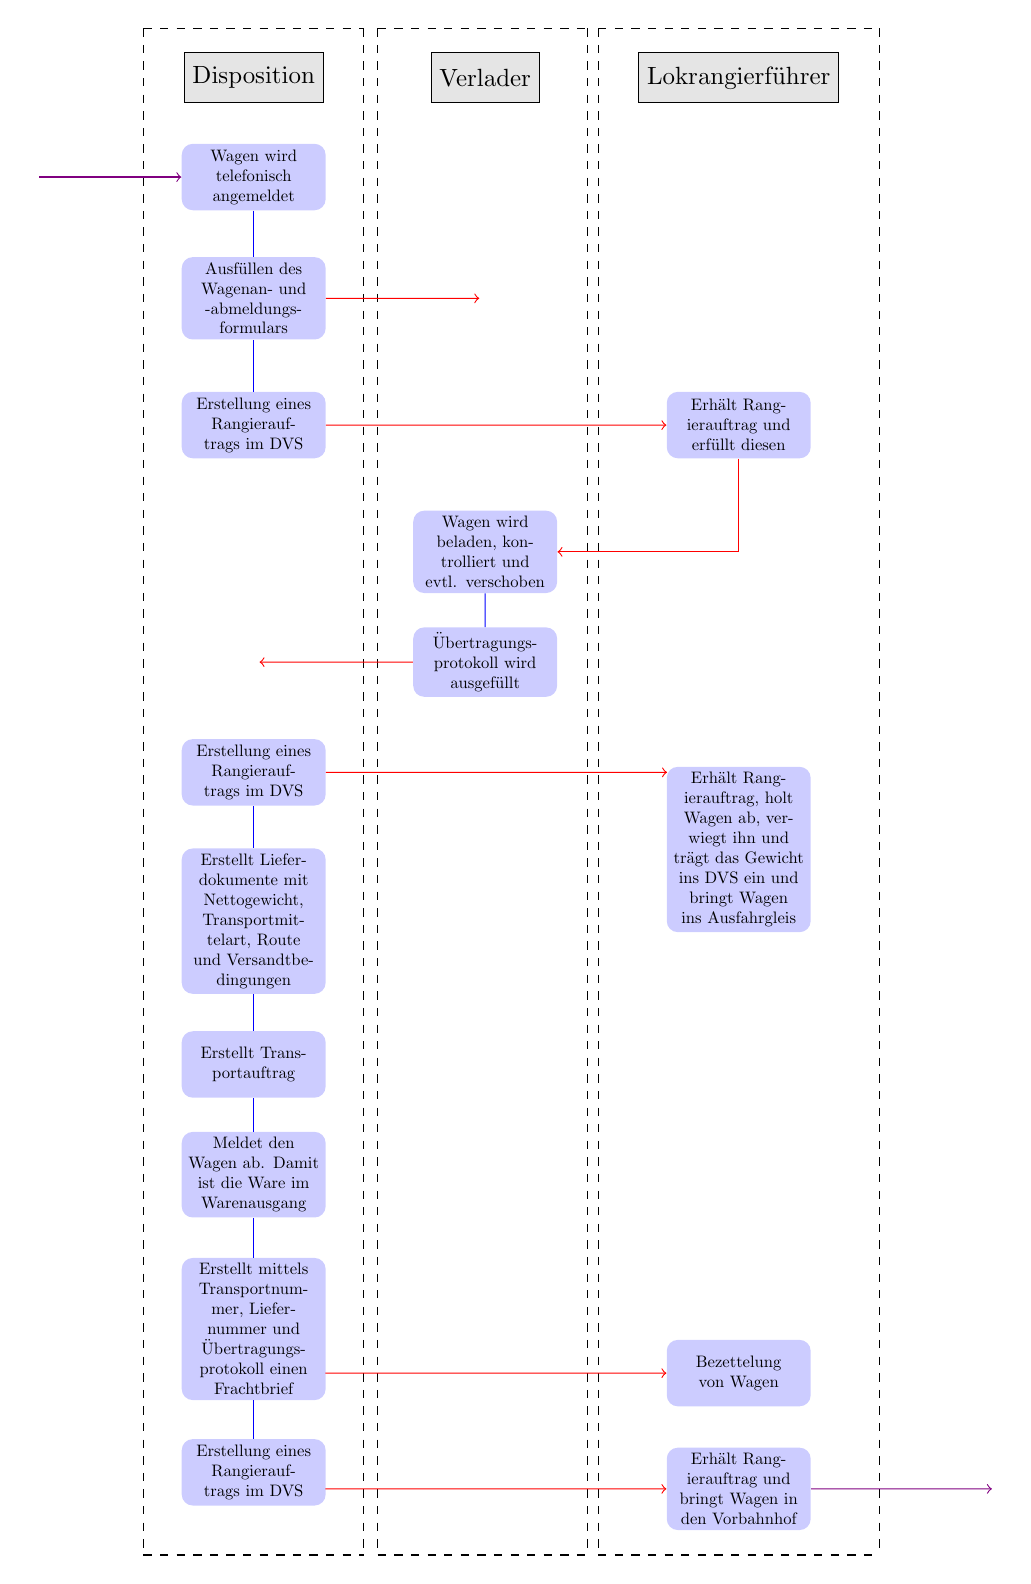
\begin{tikzpicture}[scale=0.7, every node/.style={scale=0.6}]
% Place nodes
    \node[invisible] at (-8, -1.5) (anmeldung) {};
    \node[cloud, scale=1.5] at (-4,0.3)      (dispo)         {Disposition};
    \node[cloud, scale=1.5] at (0.2, 0.3)      (verlader)      {Verlader} ;
    \node[cloud, scale=1.5] at (4.8,0.3)       (rangierende)   {Lokrangierführer};
        \node[invisible] at (-8, -1.5) (anmeldung) {};
    \node[block] at (-4, -1.5)  (Wagen)         {Wagen wird telefonisch angemeldet};
    \node[block] at (-4, -3.7)  (Waamf)         {Ausfüllen des Wagenan- und -abmeldungs- formulars};
        \node[invisible] at (0.2, -3.7) (vInfo) {};
    \node[block] at (-4, -6)    (RA)            {Erstellung eines Rangierauftrags im DVS};
    \node[block] at (4.8, -6)     (RA2)           {Erhält Rangierauftrag und erfüllt diesen};
    \node[block] at (0.2, -8.3)   (beladung)      {Wagen wird beladen, kontrolliert und evtl. verschoben};
    \node[block] at (0.2, -10.3)  (ueprot)        {Übertragungs- protokoll wird ausgefüllt};
        \node[invisible] at (-4, -10.3) (dInfo) {};
    \node[block] at (-4, -12.3) (RA3)           {Erstellung eines Rangierauftrags im DVS};
    \node[block] at (4.8, -13.7)  (RA4)           {Erhält Rangierauftrag, holt Wagen ab, verwiegt ihn und trägt das Gewicht ins DVS ein und bringt Wagen ins Ausfahrgleis};
    \node[block] at (-4, -15)   (Lieferdoc)     {Erstellt Lieferdokumente mit Nettogewicht, Transportmittelart, Route und Versandtbedingungen};
    \node[block] at (-4, -17.6) (Transportdoc)  {Erstellt Transportauftrag};
    \node[block] at (-4, -19.6) (abmelden)      {Meldet den Wagen ab. Damit ist die Ware im Warenausgang};
    \node[block] at (-4, -22.4) (Frachtbrief)   {Erstellt mittels Transportnummer, Liefernummer und Übertragungs- protokoll einen Frachtbrief};
    \node[block] at (4.8, -23.2)  (Zettel)        {Bezettelung von Wagen};
    \node[block] at (-4, -25.0) (RA5)           {Erstellung eines Rangierauftrags im DVS};
    \node[block] at (4.8, -25.3)  (RA6)           {Erhält Rangierauftrag und bringt Wagen in den Vorbahnhof};
        \node[invisible] at (9.5, -25.3) (ende) {};

% Draw edges
    %Kasten Dispo
    \draw[dashed] (-6, 1.2) -- (-6,-26.5);
    \draw[dashed] (-6, 1.2) -- (-2, 1.2);
    \draw[dashed] (-2, 1.2) -- (-2, -26.5);
    \draw[dashed] (-6, -26.5) -- (-2, -26.5);
    %Kasten Verlader
    \draw[dashed] (-1.75, 1.2) -- (2.05, 1.2);
    \draw[dashed] (-1.75, 1.2) -- (-1.75, -26.5);
    \draw[dashed] (-1.75, -26.5) -- (2.05, -26.5);
    \draw[dashed] (2.05, 1.2) -- (2.05, -26.5);
    %Kasten LRF
    \draw[dashed] (2.25, 1.2) -- (2.25, -26.5);
    \draw[dashed] (2.25, 1.2) -- (7.35, 1.2);
    \draw[dashed] (2.25, -26.5) -- (7.35, -26.5);
    \draw[dashed] (7.35, 1.2) -- (7.35, -26.5);
    
    %Pfeile ohne Beginn
    \draw[->, color=violet] (anmeldung) -- (Wagen);
    %Pfeile ohne Ende 
    \draw[->, color=red] (Waamf) -- (vInfo);
    \draw[->, color=red] (ueprot) -- (dInfo);
    \draw[->, color=violet] (RA6) -- (ende);
    %Pfeile mit Ende
    \draw[-, color=blue!100] (Wagen) -- (Waamf);
    \draw[-, color=blue] (Waamf) -- (RA);
    \draw[->, color=red] (RA) -- (RA2);
    \draw[->, color=red] (RA2) |- (beladung);
    \draw[-, color=blue] (beladung) -- (ueprot);
    \draw[->, color=red] (RA3) -- (3.5, -12.3);
    \draw[-, color=blue] (RA3) -- (Lieferdoc);
    \draw[-, color=blue] (Lieferdoc) -- (Transportdoc);
    \draw[-, color=blue] (Transportdoc) -- (abmelden);
    \draw[-, color=blue] (abmelden) -- (Frachtbrief);
    \draw[->, color=red] (-2.7, -23.2) -- (Zettel);
    \draw[-, color=blue] (Frachtbrief) -- (RA5);
    \draw[->, color=red] (-2.7, -25.3) -- (RA6);
    
\end{tikzpicture}

    \caption{Caption Wagenausgang}
    \label{fig:IDR_Warenausgang}
\end{figure}
%Der Wagen wird telefonisch bei der Disposition angemeldet, die ein Formular zur Wagenan- und Wagenabmeldung für die Abfüllung ausfüllt. Danach wird ein Rangierauftrag zum Abfüllgleis erstellt.